\documentclass{article}
% Some basic packagesLLuu
\usepackage[utf8]{inputenc}
\usepackage{spverbatim}
\usepackage[margin=1.2in]{geometry}
\usepackage{textcomp}
\usepackage{url}
\usepackage{graphicx}
\usepackage{float}
\usepackage{enumitem}
\usepackage{standalone}
\usepackage{tcolorbox}
\usepackage{wrapfig}
% \usepackage{svg}
% \usepackage{svg-inkscape} 

\graphicspath{{./figures}}

%color settings
\usepackage{xcolor}
\definecolor{gruvbgdark}{HTML}{1d2021}
\definecolor{gruvtextdark}{HTML}{ebdbb2}
\definecolor{gruvbglight}{HTML}{f9f5d7}
\definecolor{gruvtextlight}{HTML}{3c3836}
\definecolor{NavyBlue}{HTML}{266bbd}
\definecolor{RawSienna}{HTML}{94330e}
\definecolor{ForestGreen}{HTML}{149b52}
% \pagecolor{gruvbgdark}
% \color{gruvtextdark}

% Hide page number when page is empty
\usepackage{emptypage}
\usepackage{subcaption}
\usepackage{multicol}

% Math stuff
\usepackage{amsmath, amsfonts, mathtools, amsthm, amssymb}
% Fancy script capitals
\usepackage{mathrsfs}
\usepackage{cancel}

% Bold math
\usepackage{bm}

% SVG setup
% \svgsetup{inkscapeexe=inkscape, inkscapearea=drawing}
% \svgpath{~/dev/DAVE3700-Matte-3000/figures/}

% Some shortcuts
\newcommand\N{\ensuremath{\mathbb{N}}}
\newcommand\R{\ensuremath{\mathbb{R}}}
\newcommand\Z{\ensuremath{\mathbb{Z}}}
\renewcommand\O{\ensuremath{\emptyset}}
\newcommand\Q{\ensuremath{\mathbb{Q}}}
\newcommand\C{\ensuremath{\mathbb{C}}}

%Make implies and impliedby shorter
\let\implies\Rightarrow
\let\impliedby\Leftarrow
\let\iff\Leftrightarrow

\let\epsilon\varepsilon

% Add \contra symbol to denote contradiction
% \usepackage{stmaryrd} % for \lightning
% \newcommand\contra{\scalebox{1.5}{$\lightning$}}

\let\phi\varphi

% Command for short corrections
% Usage: 1+1=\correct{3}{2}

\definecolor{correct}{HTML}{009900}
\newcommand\correct[2]{\ensuremath{\:}{\color{red}{#1}}\ensuremath{\to }{\color{correct}{#2}}\ensuremath{\:}}
\newcommand\green[1]{{\color{correct}{#1}}}

% horizontal rule
% \newcommand\hr{
%     \noindent\rule[0.5ex]{\linewidth}{0.5pt}
% }

% hide parts
\newcommand\hide[1]{}

% Environments
\makeatother

% For box around Definition, Theorem, \ldots
% theorems
\usepackage{thmtools}
\usepackage[framemethod=TikZ]{mdframed}
\mdfsetup{skipabove=1em,skipbelow=1em, innertopmargin=5pt, innerbottommargin=6pt}

\theoremstyle{definition}

\makeatletter

% \declaretheoremstyle[headfont=\bfseries, bodyfont=\normalfont, mdframed={ nobreak } ]{thmgreenbox}
% \declaretheoremstyle[headfont=\bfseries, bodyfont=\normalfont, mdframed={ nobreak } ]{thmredbox}
% \declaretheoremstyle[headfont=\bfseries, bodyfont=\normalfont, spaceabove=0.5cm, spacebelow=0.5cm]{thmbluebox}
% % \declaretheoremstyle[headfont=\bfseries, bodyfont=\normalfont]{thmbluebox}
% \declaretheoremstyle[headfont=\bfseries, bodyfont=\normalfont]{thmblueline}
% \declaretheoremstyle[headfont=\bfseries, bodyfont=\normalfont, numbered=no, mdframed={ rightline=false, topline=false, bottomline=false, }, qed=\qedsymbol ]{thmproofbox}
% \declaretheoremstyle[headfont=\bfseries\sffamily, bodyfont=\normalfont, numbered=no, mdframed={ nobreak, rightline=false, topline=false, bottomline=false } ]{thmexplanationbox}
\declaretheoremstyle[headfont=\bfseries, bodyfont=\normalfont, numbered=no]{idea}

\declaretheoremstyle[
	headfont=\bfseries\color{ForestGreen!70!black}, bodyfont=\normalfont,
	mdframed={
			linewidth=2pt,
			rightline=false, topline=false, bottomline=false,
			linecolor=ForestGreen, backgroundcolor=ForestGreen!5,
		}
]{thmgreenbox}

\declaretheoremstyle[
	headfont=\bfseries\color{NavyBlue!70!black}, bodyfont=\normalfont,
	mdframed={
			linewidth=2pt,
			rightline=false, topline=false, bottomline=false,
			linecolor=NavyBlue, backgroundcolor=NavyBlue!5,
		}
]{thmbluebox}

\declaretheoremstyle[
	headfont=\bfseries\color{NavyBlue!70!black}, bodyfont=\normalfont,
	mdframed={
			linewidth=2pt,
			rightline=false, topline=false, bottomline=false,
			linecolor=NavyBlue
		}
]{thmblueline}

\declaretheoremstyle[
	headfont=\bfseries\color{RawSienna!70!black}, bodyfont=\normalfont,
	mdframed={
			linewidth=2pt,
			rightline=false, topline=false, bottomline=false,
			linecolor=RawSienna, backgroundcolor=RawSienna!5,
		}
]{thmredbox}

\declaretheoremstyle[
	headfont=\bfseries\color{RawSienna!70!black}, bodyfont=\normalfont,
	numbered=no,
	mdframed={
			linewidth=2pt,
			rightline=false, topline=false, bottomline=false,
			linecolor=RawSienna, backgroundcolor=RawSienna!5,
		},
	qed=\qedsymbol
]{thmproofbox}

\declaretheoremstyle[
	headfont=\bfseries\color{NavyBlue!70!black}, bodyfont=\normalfont,
	numbered=no,
	mdframed={
			linewidth=2pt,
			rightline=false, topline=false, bottomline=false,
			linecolor=NavyBlue, backgroundcolor=NavyBlue!1,
		},
]{thmexplanationbox}

\declaretheorem[style=thmgreenbox, name=Definisjon]{definition}
\declaretheorem[sibling=definition, style=thmredbox, name=Corollary]{corollary}
\declaretheorem[style=thmbluebox, numbered=no, name=Idea]{idea}
\declaretheorem[style=idea, style=thmredbox, name=Proposition]{prop}
\declaretheorem[sibling=definition, style=thmredbox, name=Theorem]{theorem}
\declaretheorem[sibling=definition, style=thmredbox, name=Lemma]{lemma}



\declaretheorem[numbered=no, style=thmexplanationbox, name=Proof]{explanation}
\declaretheorem[numbered=no, style=thmproofbox, name=Bevis]{replacementproof}
\declaretheorem[style=thmgreenbox,  numbered=no, name=Oppgave]{ex}
\declaretheorem[style=thmbluebox,  numbered=no, name=Eksempel]{eg} \declaretheorem[style=thmblueline, numbered=no, name=Remark]{remark}
\declaretheorem[style=thmblueline, numbered=no, name=Merk]{note}

\renewenvironment{proof}[1][\proofname]{\begin{replacementproof}}{\end{replacementproof}}

\AtEndEnvironment{eg}{\null\hfill$\diamond$}%

\newtheorem*{uovt}{UOVT}
\newtheorem*{notation}{Notation}
\newtheorem*{previouslyseen}{As previously seen}
\newtheorem*{problem}{Problem}
\newtheorem*{observe}{Observe}
\newtheorem*{property}{Property}
\newtheorem*{intuition}{Intuition}


% Exercise 
% Usage:
% \oefening{5}
% \suboefening{1}
% \suboefening{2}
% \suboefening{3}
% gives
% Oefening 5
%   Oefening 5.1
%   Oefening 5.2
%   Oefening 5.3
\newcommand{\oefening}[1]{%
	\def\@oefening{#1}%
	\subsection*{Oefening #1}
}

\newcommand{\suboefening}[1]{%
	\subsubsection*{Oefening \@oefening.#1}
}


% \lecture starts a new lecture (les in dutch)
%
% Usage:
% \lecture{1}{di 12 feb 2019 16:00}{Inleiding}
%
% This adds a section heading with the number / title of the lecture and a
% margin paragraph with the date.

% I use \dateparts here to hide the year (2019). This way, I can easily parse
% the date of each lecture unambiguously while still having a human-friendly
% short format printed to the pdf.

% \usepackage{xifthen}
% \def\testdateparts#1{\dateparts#1\relax}
% \def\dateparts#1 #2 #3 #4 #5\relax{
% 	\marginpar{\small\textsf{\mbox{#1 #2 #3 #5}}}
% }

% \def\@lecture{}%
% \newcommand{\lecture}[3]{
% 	\ifthenelse{\isempty{#3}}{%
% 		\def\@lecture{Lecture #1}%
% 	}{%
% 		\def\@lecture{Lecture #1: #3}%
% 	}%
% 	\subsection*{\@lecture}
% 	% \marginpar{\small\textsf{\mbox{#2}}}
% }

\usepackage{listings}

\definecolor{dkgreen}{rgb}{0,0.6,0}
\definecolor{gray}{rgb}{0.5,0.5,0.5}
\definecolor{mauve}{rgb}{0.58,0,0.82}

\lstset{frame=none,
  language=Haskell,
  aboveskip=3mm,
  belowskip=3mm,
  showstringspaces=false,
  columns=flexible,
  basicstyle={\small\ttfamily},
  numbers=none,
  numberstyle=\tiny\color{gray},
  keywordstyle=\color{blue},
  commentstyle=\color{dkgreen},
  stringstyle=\color{mauve},
  breaklines=true,
  breakatwhitespace=true,
  tabsize=3
}



% These are the fancy headers
\usepackage{fancyhdr}
\pagestyle{fancy}

% LE: left even
% RO: right odd
% CE, CO: center even, center odd
% My name for when I print my lecture notes to use for an open book exam.
\fancyhead[LE,RO]{Kristian Sørdal}

\fancyhead[RO,LE]{INF122 - Funksjonell Programmering} % Right odd,  Left even
% \fancyhead[RE,LO]{\leftmark}          % Right even, Left odd
\fancyhead[RE,LO]{Kristian Sørdal}          % Right even, Left odd

\fancyfoot[RO,LE]{\thepage}  % Right odd,  Left even
% \fancyfoot[RE,LO]{Kristian Sørdal}          % Right even, Left odd
\fancyfoot[C]{\leftmark}     % Center

\makeatother

% Todonotes and inline notes in fancy boxes
\usepackage{todonotes}
\usepackage{tcolorbox}

% Make boxes breakable
\tcbuselibrary{breakable}

% Figure support as explained in my blog post.
\usepackage{import}
\usepackage{xifthen}
\usepackage{pdfpages}
\usepackage{transparent}
\newcommand{\incfig}[2][1]{%
	% \begin{center}
	\def\svgwidth{#1\columnwidth}
	\import{./figures/}{#2.pdf_tex}
	% \end{center}
}
% Fix some stuff
% %http://tex.stackexchange.com/questions/76273/multiple-pdfs-with-page-group-included-in-a-single-page-warning
\pdfsuppresswarningpagegroup=1
\author{Kristian Sørdal}


\begin{document}
    \section{Forelesning 10}

    \subsection{Plan for forelesningen}
    \begin{itemize}
        \item Induktive datastrukturer
        \item AVL trær
        \item Syntakstrær
    \end{itemize}

   \subsection{Induktive data strukturer}
   En datastruktur er induktiv hvis den bruker seg selv som argument til minst en av konstruktørene.

    \begin{lstlisting}
    data binTree a = Empty
        | Branch (BinTree a) a (BinTree a)
    \end{lstlisting}    

    ELementene i en induktiv datastruktur kan settes sammen ved hjelp av konstrukt;rene til store strukturer (trær)

    \subsection{Rekursjon på induktive datastrukturer}
    For å definere en funksjon som tar en indktiv struktur som argumen ved rekursjon

    \begin{itemize}
        \item Gjøre mønster matching på funksjonen:
            \begin{itemize}
                \item Lag et tilfelle for hver konstruktør
                \item Argumentene til konstruktøren blir variabler
            \end{itemize}
        \item Definer funksjonen i hvert tilfelle
        \item Kall funksjonen rekursivt på de variblene som igjen er elementer av den induktive datastrukturen
    \end{itemize}   

    \begin{eg}
        La oss beregne høyden av et binært tre

    \begin{lstlisting}
    height :: BinTree a -> Integer
    height Empty = 0
    height (Branch lefts _ rights)
        = 1 + max (height lefts) (height rights)
    \end{lstlisting}

    Følger denne funksjonen oppskriften fra forrige slide?
    \end{eg}


    \begin{figure}[H]
        \begin{center}
            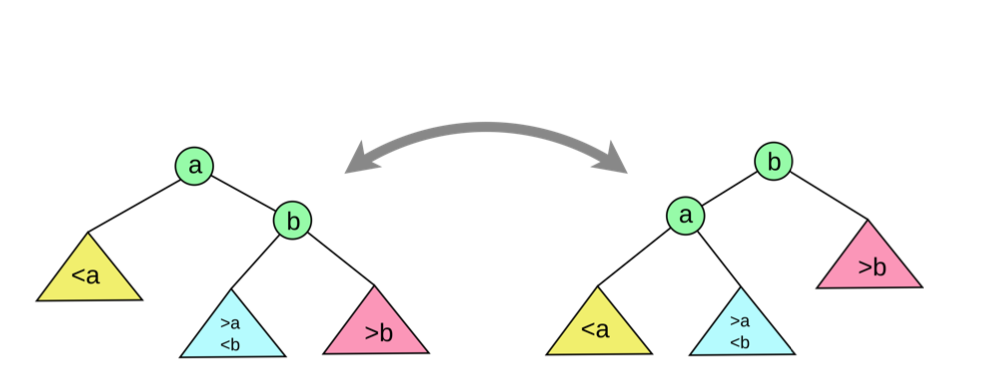
\includegraphics[width=0.95\textwidth]{rotasjontree}
        \end{center}
        \caption{Illustrasjon av rotasjonsoperasjonen}
        \label{fig:rotasjontree}
    \end{figure}

    \subsection{Rotasjon av trær}
    Et tre kan roteres mot høyre, eller mot venstre, og en rotasjon kan endre høyden til treet.
    \begin{eg}
        Rotasjon av trær
       \begin{figure}[H]
           \begin{center}
               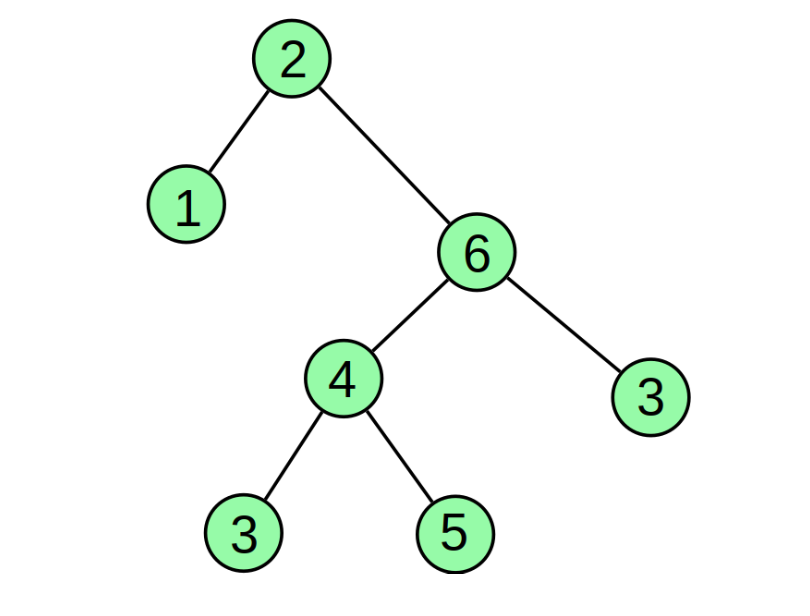
\includegraphics[width=0.65\textwidth]{rotationexample}
           \end{center}
           \caption{Bruk rotasjonsoperasjoner til å balansere treet.}
           \label{fig:rotationexample}
       \end{figure} 

       \begin{figure}[H]
        \centering
        \incfig{rotatetree}
        \end{figure}
    \end{eg}

    \subsection{AVL Trær}
    \begin{itemize}
        \item Introdusert av Adelson-Velsky og Landig i 1962
        \item Består av et binært tre med ekstra balanse informasjon
        \item Definerer et API p3l binære trær som roterer hver gang en ubalanse oppstår
    \end{itemize}

    \subsection{AVL Trær: Implementasjon}
    AVL trær har en balanseinvariant
    \begin{itemize}
        \item Ingen subtrær kan ha en høydeforskjell på mer enn 1.    
        \item En hver forgening er dekorert med høydeforskjellen på de to subtrærne. Denne kalles \textbf{balansefaktoren}.
    \end{itemize}

    \begin{ex}
        Som en øvelse før vi gjør AVL trær, så implementerer vi sorterte lister, dekorert med om de er av odde eller partalls lengde.
    \end{ex}

    \newpage

    \subsection{AVL Datatypen}    
    \begin{lstlisting}
     data BalanceFactor = LeftHeavy
                        | Balanced
                        | RightHeavy
                        deriving (Eq, Show)
    data AVLTree a = Empty
                   | Branch BalanceFactor
                            (AVLTree a)
                            a
                            (AVLTree a)
    \end{lstlisting}
\end{document}
